\documentclass[12pt]{article}
\usepackage[margin=1in]{geometry}
\usepackage{amsmath}
\usepackage{amssymb}
\usepackage{graphicx}
\usepackage{booktabs}
\usepackage{hyperref}
\usepackage[capitalise]{cleveref}
\usepackage{microtype}
\usepackage{parskip}

\graphicspath{{images/}}

\newcommand{\figplaceholder}[2][3in]{%
  \begin{center}
  \fbox{\parbox{#1}{\centering\vspace{0.5in}\textit{[Figure: #2]}\vspace{0.5in}}}
  \end{center}
}

\title{Time Response\\[0.5em]
\large ME 2801 --- Week 4}
\author{}
\date{}

\begin{document}
\maketitle
\tableofcontents
\newpage

% ===========================================================================
\section{Multiple Lenses on a Dynamic System}
\label{sec:intro}
% ===========================================================================

By now we have built up several ways of looking at a dynamic system.  Each
represents the same underlying physics, but each brings different structure
into focus:

\begin{itemize}
  \item \textbf{Governing equations (ODE).}  The direct mathematical model ---
    Newton's second law, Kirchhoff's laws, etc.  Precise, but solving it for
    every input becomes tedious.
  \item \textbf{Transfer function} $G(s)$.  The Laplace-domain input/output
    relationship.  Turns convolution into multiplication and makes block diagrams
    possible.
  \item \textbf{Pole-zero map.}  A visual representation of $G(s)$ in the
    complex $s$-plane.  Poles govern the character of the natural response;
    poles and zeros together set amplitudes.
  \item \textbf{Time response.}  The actual output $c(t)$ as a function of
    time for a defined input --- the most direct view for engineers who need
    to specify and measure system behavior.
\end{itemize}

These views complement one another.  A skilled controls engineer moves
fluently between them, using whichever lens is most convenient for the task at
hand.  Figure~\ref{fig:views} captures this theme: for a second-order system,
the pole location, the time response shape, and the system parameters are
all different expressions of the same underlying dynamics.

\begin{figure}[h]
  \centering
  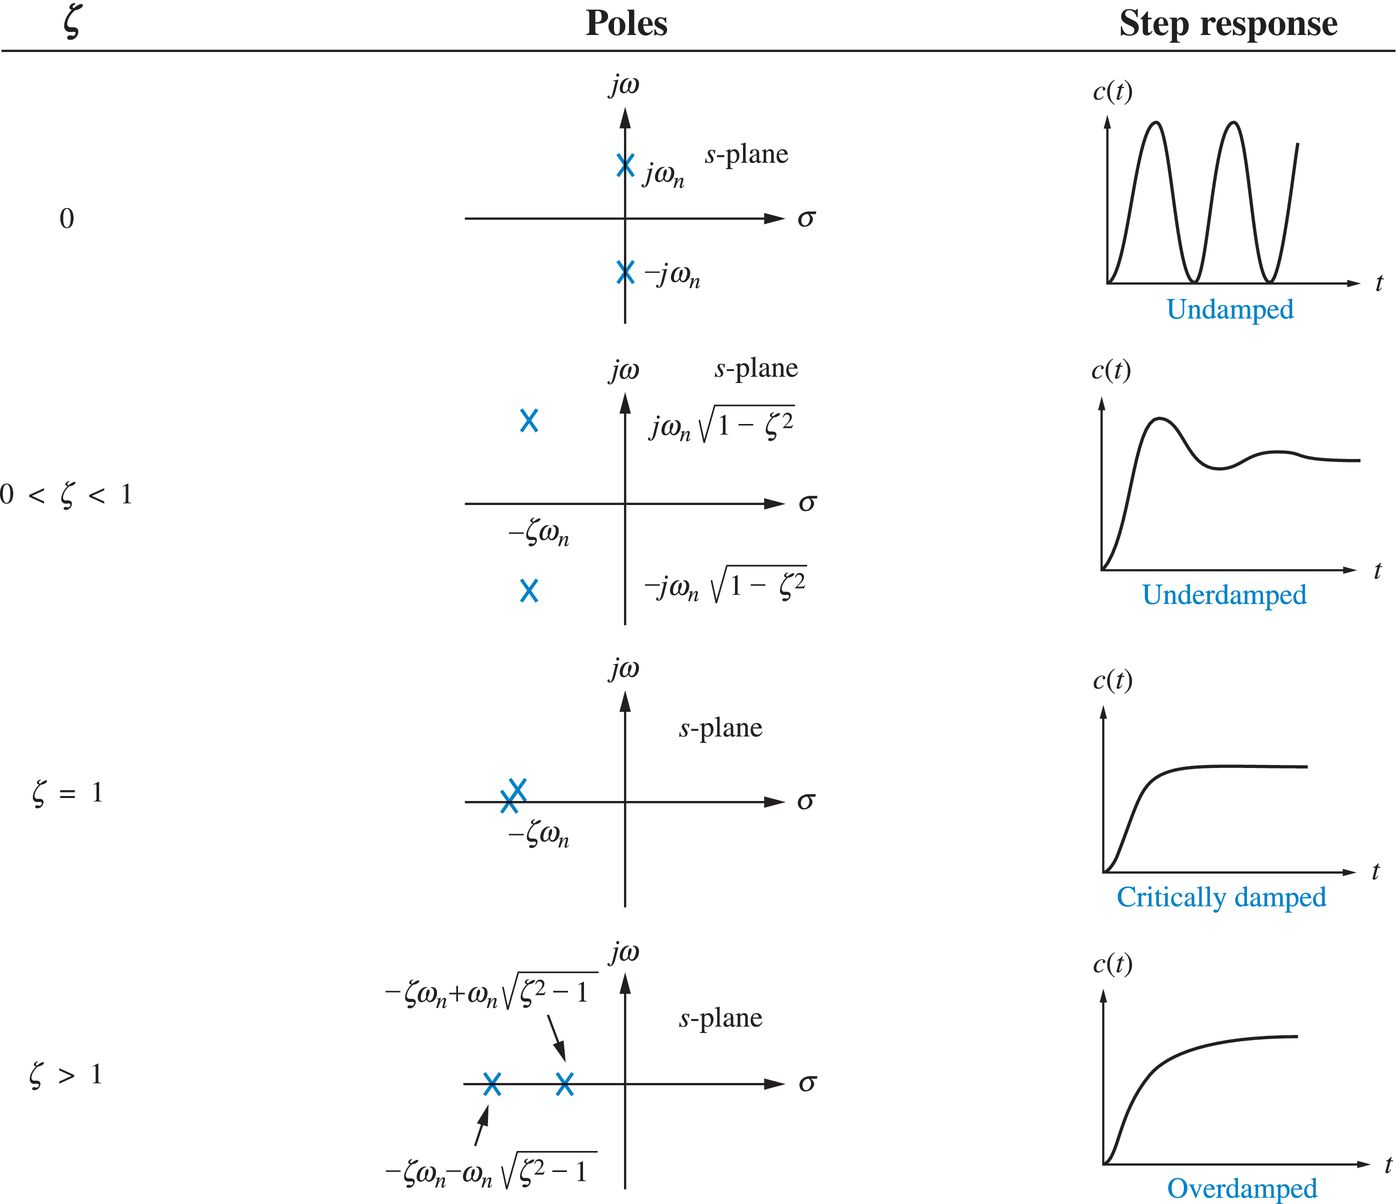
\includegraphics[width=0.75\textwidth]{fig_04_11.jpg}
  \caption{Second-order step response as a function of damping ratio~$\zeta$.
    Each row shows the same dynamics through three lenses: the value of~$\zeta$,
    the pole location in the $s$-plane, and the step response shape.
    (Adapted from Nise, Fig.~4.11.)}
  \label{fig:views}
\end{figure}

This week focuses on the time response.  We analyze first- and second-order
systems in detail because they are the \emph{building blocks} of all linear
systems.

% ===========================================================================
\section{Building Blocks: Why First and Second Order?}
\label{sec:blocks}
% ===========================================================================

Any rational transfer function can be expanded via partial fractions into a
sum of simpler terms.  The possible building blocks are:

\begin{center}
\begin{tabular}{lll}
  \toprule
  Block type & Transfer function & Time response \\
  \midrule
  Gain & $K$ & instantaneous scaling \\
  Integrator / differentiator & $1/s$, $s$ & ramp, impulse \\
  First-order & $\dfrac{a}{s+a}$ & decaying exponential \\
  Second-order (underdamped) & $\dfrac{\omega_d^2+\sigma_d^2}{(s+\sigma_d)^2+\omega_d^2}$ &
    exponentially decaying sinusoid \\
  \bottomrule
\end{tabular}
\end{center}

Because Laplace transforms turn convolution into multiplication, a complex
transfer function that is a \emph{product} of building blocks corresponds to
a cascade (series) connection in block diagrams.  Once we understand the
response of each building block, we have the intuition to understand any
LTI system.

Underdamped second-order blocks deserve special attention because they produce
the rich transient behavior --- overshoot, ringing, oscillation --- that
dominates practical control design.

% ===========================================================================
\section{First-Order Systems}
\label{sec:first}
% ===========================================================================

% ---------------------------------------------------------------------------
\subsection{Canonical Forms}
\label{sec:first_forms}
% ---------------------------------------------------------------------------

A first-order system without zeros has the transfer function

\begin{equation}
  G_1(s) = \frac{K_{dc}}{\tau s + 1} = K_{dc}\,\frac{a}{s+a}
  \label{eq:G1}
\end{equation}

where $a = 1/\tau$.  Both forms carry identical information, but each
highlights something different:

\begin{itemize}
  \item \textbf{Time-constant form} $K_{dc}/(\tau s+1)$: the parameter~$\tau$
    (the \emph{time constant}) is immediately visible.  At $s=0$ the function
    evaluates to $K_{dc}$, confirming the DC gain.
  \item \textbf{Pole form} $K_{dc}\,a/(s+a)$: the pole is at $s = -a$.  The
    exponential frequency of the natural response equals~$a$, so a pole farther
    from the imaginary axis (larger~$a$) means a faster transient decay.
\end{itemize}

% ---------------------------------------------------------------------------
\subsection{Step Response}
\label{sec:first_step}
% ---------------------------------------------------------------------------

For a unit step input, $R(s) = 1/s$, the output transform is

\[
  C(s) = G_1(s)\,\frac{1}{s} = K_{dc}\,\frac{a}{s(s+a)}
       = K_{dc}\left(\frac{1}{s} - \frac{1}{s+a}\right)
\]

Taking the inverse Laplace transform gives the step response

\begin{equation}
  \boxed{c(t) = K_{dc}\!\left(1 - e^{-at}\right) = K_{dc}\!\left(1 - e^{-t/\tau}\right)}
  \label{eq:first_step}
\end{equation}

The response is a rising exponential that approaches the steady-state value
$K_{dc}$ --- the DC gain.  The shape is set entirely by~$\tau$; changing $\tau$
stretches or compresses the time axis without changing the character of the
response.

\begin{figure}[h]
  \centering
  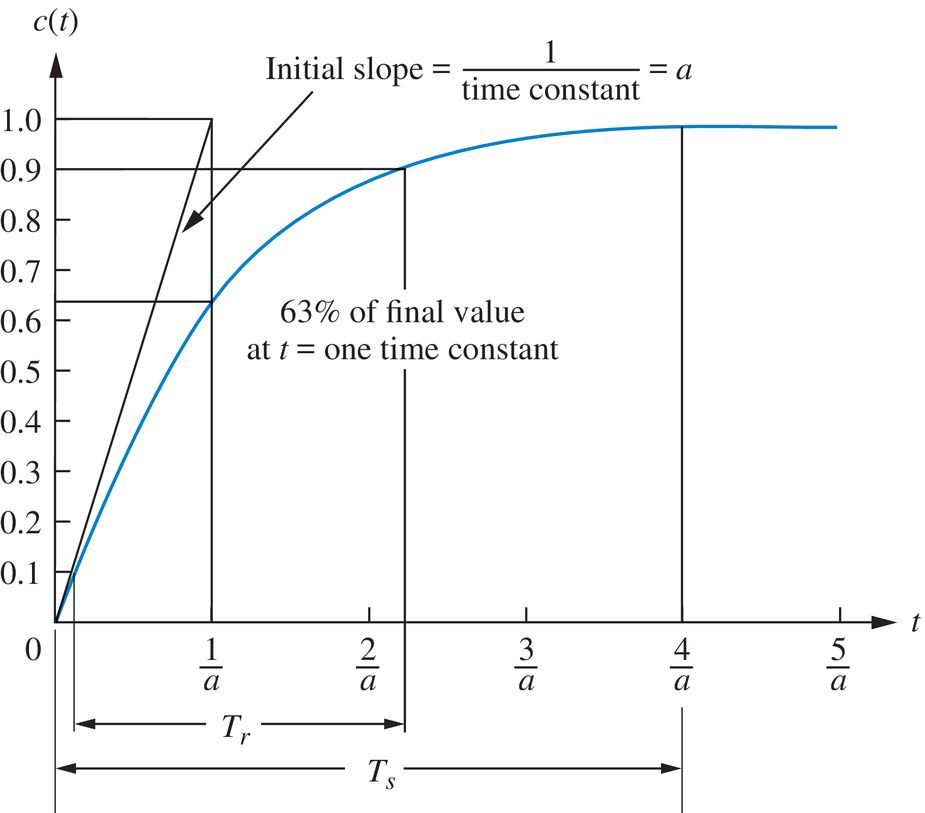
\includegraphics[width=0.6\textwidth]{fig_04_05.jpg}
  \caption{Unit step response of a first-order system, illustrating the time
    constant~$\tau$, rise time~$T_r$, and settling time~$T_s$.
    (Adapted from Nise, Fig.~4.5.)}
  \label{fig:first_step}
\end{figure}

% ---------------------------------------------------------------------------
\subsection{System Parameters: DC Gain and Time Constant}
\label{sec:first_params}
% ---------------------------------------------------------------------------

A first-order system is fully characterized by two parameters:

\begin{description}
  \item[$K_{dc}$ (DC gain)] The steady-state output magnitude for a unit step.
    Read directly from the transfer function as $G_1(0) = K_{dc}$.
  \item[$\tau$ (time constant)] The characteristic time of the exponential
    decay.  It sets the speed of the response.  Equivalently, $\tau$ is the
    reciprocal of the pole location: $\tau = 1/a$.
\end{description}

% ---------------------------------------------------------------------------
\subsection{Transient Performance Metrics}
\label{sec:first_metrics}
% ---------------------------------------------------------------------------

Three standard metrics describe the speed of a first-order step response.
All follow directly from Eq.~\eqref{eq:first_step}.

\begin{description}
  \item[Time constant~$\tau$] At $t = \tau$, the response reaches
    $1 - e^{-1} \approx 63\%$ of $K_{dc}$.
    This is the most fundamental speed measure for a first-order system.

  \item[Rise time~$T_r$] Time to go from 10\% to 90\% of the final value.
    Setting $c(t) = 0.1\,K_{dc}$ and $c(t) = 0.9\,K_{dc}$ and taking the
    difference:
    \begin{equation}
      T_r = \frac{2.2}{a} = 2.2\,\tau
      \label{eq:first_tr}
    \end{equation}

  \item[Settling time~$T_s$] Time for the response to remain within 2\% of
    its final value.  Setting $|1 - c(t)/K_{dc}| = 0.02$ gives
    \begin{equation}
      T_s = \frac{4}{a} = 4\,\tau
      \label{eq:first_ts}
    \end{equation}
\end{description}

% ---------------------------------------------------------------------------
\subsection{Pole Location and Response Speed}
\label{sec:first_pole}
% ---------------------------------------------------------------------------

The pole of $G_1(s)$ is at $s = -a = -1/\tau$.  The connection is direct:
\begin{itemize}
  \item A pole \emph{farther from the imaginary axis} (larger~$|a|$, smaller
    $\tau$) means a faster transient --- $T_r$ and $T_s$ both decrease.
  \item A pole \emph{closer to the imaginary axis} means a slower transient.
  \item A pole \emph{on the imaginary axis} ($a = 0$) gives an integrator ---
    no steady state for a step input.
\end{itemize}

This pole-to-speed connection generalizes to all LTI systems: the real part
of a pole determines the rate of exponential decay of that response component.

% ===========================================================================
\section{Second-Order Systems}
\label{sec:second}
% ===========================================================================

% ---------------------------------------------------------------------------
\subsection{Canonical Forms}
\label{sec:second_forms}
% ---------------------------------------------------------------------------

The canonical second-order transfer function is written in two equivalent forms:

\begin{equation}
  G_2(s)
    = K_{dc}\,\frac{\omega_n^2}{s^2 + 2\zeta\omega_n s + \omega_n^2}
    = K_{dc}\,\frac{\sigma_d^2 + \omega_d^2}{(s+\sigma_d)^2 + \omega_d^2}
  \label{eq:G2}
\end{equation}

where the system parameters are:

\begin{center}
\begin{tabular}{lll}
  \toprule
  Symbol & Name & Meaning \\
  \midrule
  $K_{dc}$ & DC gain & steady-state output per unit step input \\
  $\omega_n$ & natural frequency & oscillation frequency with no damping \\
  $\zeta$ & damping ratio & shape of transient (see below) \\
  $\sigma_d = \zeta\omega_n$ & exponential damping frequency &
    rate of exponential envelope decay \\
  $\omega_d = \omega_n\sqrt{1-\zeta^2}$ & damped natural frequency &
    actual oscillation frequency in the transient \\
  \bottomrule
\end{tabular}
\end{center}

The two forms again emphasize different things:

\begin{itemize}
  \item \textbf{Standard form} $\omega_n^2/(s^2 + 2\zeta\omega_n s + \omega_n^2)$:
    match coefficients to read off $\omega_n$ and $\zeta$ directly.
    The denominator is the characteristic polynomial whose roots are the poles.
  \item \textbf{Pole form} $(\sigma_d^2+\omega_d^2)/[(s+\sigma_d)^2+\omega_d^2]$:
    the complex poles $s = -\sigma_d \pm j\omega_d$ are explicit.  The real
    part~$\sigma_d$ controls the \emph{exponential envelope} (how fast the
    oscillations decay), and the imaginary part~$\omega_d$ controls the
    \emph{oscillation frequency} (how fast the sinusoid cycles).
\end{itemize}

Both identities hold because $\sigma_d^2 + \omega_d^2 = (\zeta\omega_n)^2 +
\omega_n^2(1-\zeta^2) = \omega_n^2$.  Setting $s=0$ in either form gives
$G_2(0) = K_{dc}$, confirming the DC gain.

% ---------------------------------------------------------------------------
\subsection{Damping Cases}
\label{sec:second_cases}
% ---------------------------------------------------------------------------

The value of~$\zeta$ determines the character of the response.  The four cases
are summarized in Figure~\ref{fig:damping_cases} and Table~\ref{tab:cases}.

\begin{figure}[h]
  \centering
  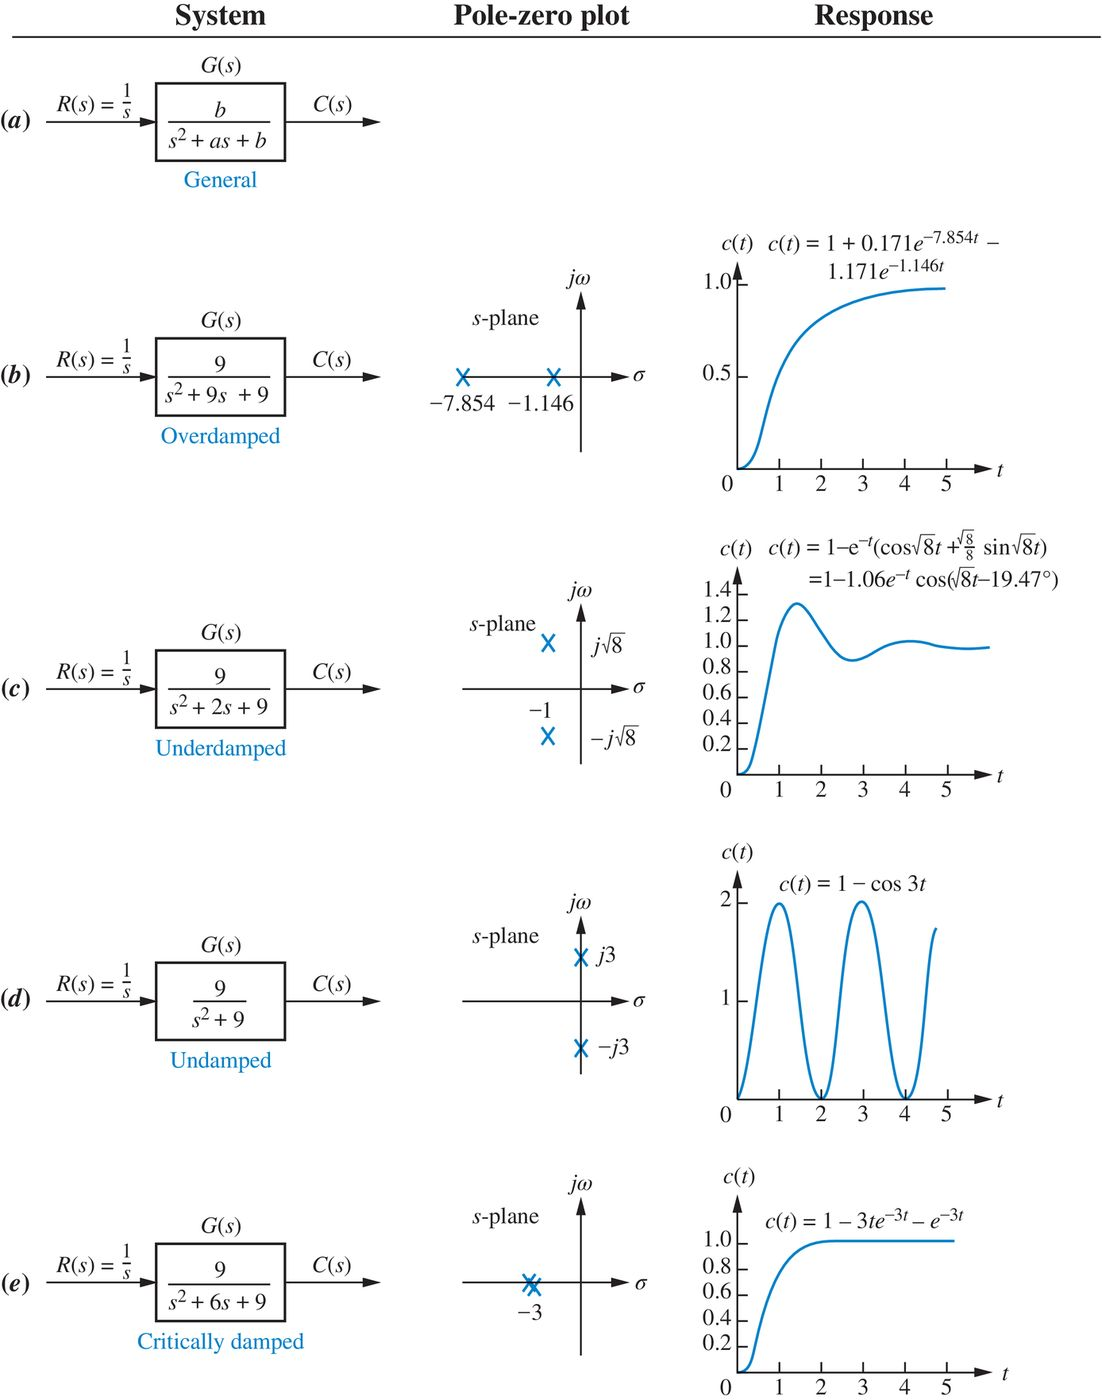
\includegraphics[width=0.85\textwidth]{fig_04_07.jpg}
  \caption{Second-order systems: pole locations and unit step responses for the
    four damping cases.
    (Adapted from Nise, Fig.~4.7.)}
  \label{fig:damping_cases}
\end{figure}

\begin{table}[h]
  \centering
  \begin{tabular}{llll}
    \toprule
    Condition & Name & Poles & Character \\
    \midrule
    $\zeta = 0$ & Undamped & $\pm\,j\omega_n$ (imaginary) &
      sustained sinusoid \\
    $0 < \zeta < 1$ & Underdamped & $-\sigma_d \pm j\omega_d$ (complex) &
      decaying sinusoid \\
    $\zeta = 1$ & Critically damped & $-\omega_n$ (repeated real) &
      fastest approach without overshoot \\
    $\zeta > 1$ & Overdamped & two distinct negative reals &
      two exponentials; sluggish \\
    \bottomrule
  \end{tabular}
  \caption{Second-order damping cases.}
  \label{tab:cases}
\end{table}

In control engineering, ``second-order system'' often implicitly means the
\emph{underdamped} case because it produces the richest behavior and the most
design-relevant transient specifications.

% ---------------------------------------------------------------------------
\subsection{Impulse Response: The Math Made Transparent}
\label{sec:second_impulse}
% ---------------------------------------------------------------------------

The step response of a second-order underdamped system requires a moderately
involved partial-fraction expansion.  The \emph{impulse response} is simpler
and reveals the same structural insight.

The Laplace transform of the impulse response is the transfer function itself,
$G_2(s)$.  Using the pole form and writing $K_{dc} = 1$ for clarity:

\[
  G_2(s) = \frac{\omega_n^2}{(s+\sigma_d)^2+\omega_d^2}
           = \frac{\omega_n^2}{\omega_d}\,\cdot\,
             \frac{\omega_d}{(s+\sigma_d)^2+\omega_d^2}
\]

The Laplace transform pair $e^{-\sigma_d t}\sin(\omega_d t)
\;\longleftrightarrow\; \omega_d/[(s+\sigma_d)^2+\omega_d^2]$ gives the
impulse response directly:

\begin{equation}
  \boxed{y_{\mathrm{imp}}(t)
    = \frac{\omega_n^2}{\omega_d}\,e^{-\sigma_d t}\sin(\omega_d t)
    = \frac{\omega_n}{\sqrt{1-\zeta^2}}\,e^{-\zeta\omega_n t}\sin(\omega_d t)}
  \label{eq:impulse}
\end{equation}

The structure is clear: a sinusoid at frequency~$\omega_d$ inside an
exponential envelope that decays at rate~$\sigma_d$.  The two parts of the
complex pole --- real part~$\sigma_d$ and imaginary part~$\omega_d$ --- map
directly and independently onto the two parts of the time response.

% ---------------------------------------------------------------------------
\subsection{Step Response}
\label{sec:second_step}
% ---------------------------------------------------------------------------

Integrating the impulse response (or inverting $G_2(s)/s$ directly) gives the
unit step response for the underdamped case:

\begin{equation}
  c(t) = K_{dc}\!\left[
    1 - \frac{1}{\sqrt{1-\zeta^2}}\,e^{-\zeta\omega_n t}
        \cos\!\left(\omega_d t - \phi\right)
  \right], \qquad
  \phi = \arctan\!\left(\frac{\zeta}{\sqrt{1-\zeta^2}}\right)
  \label{eq:step}
\end{equation}

The response again consists of a constant (the forced response) plus an
exponentially decaying sinusoid (the natural response).  Figure~\ref{fig:step_overlay}
shows unit step responses for several values of~$\zeta$; the natural frequency
$\omega_n$ sets the time scale.

\begin{figure}[h]
  \centering
  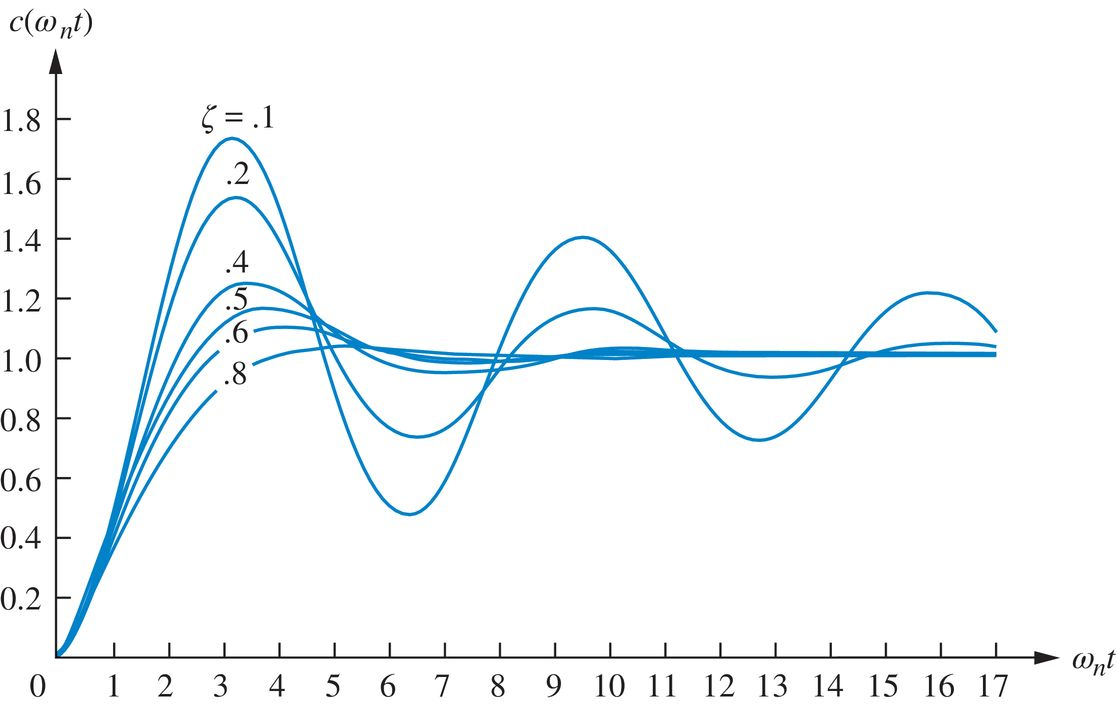
\includegraphics[width=0.65\textwidth]{fig_04_13.jpg}
  \caption{Underdamped unit step responses for various damping ratios, plotted
    on the normalized time axis~$\omega_n t$.  Decreasing~$\zeta$ increases
    both oscillation and overshoot.
    (Adapted from Nise, Fig.~4.13.)}
  \label{fig:step_overlay}
\end{figure}

% ===========================================================================
\section{Performance Metrics for Underdamped Second-Order Systems}
\label{sec:metrics}
% ===========================================================================

% ---------------------------------------------------------------------------
\subsection{The Language of Speed}
\label{sec:metrics_intro}
% ---------------------------------------------------------------------------

Transient performance metrics are the \emph{language} engineers use to
specify and measure system speed.  A requirement like ``settling time less than
0.5~s'' or ``overshoot no more than 15\%'' is far more practical than
specifying a transfer function directly.  The metrics defined here all follow
from the step response of Eq.~\eqref{eq:step}, normalized to $K_{dc} = 1$.

Figure~\ref{fig:specs} defines the four metrics graphically.

\begin{figure}[h]
  \centering
  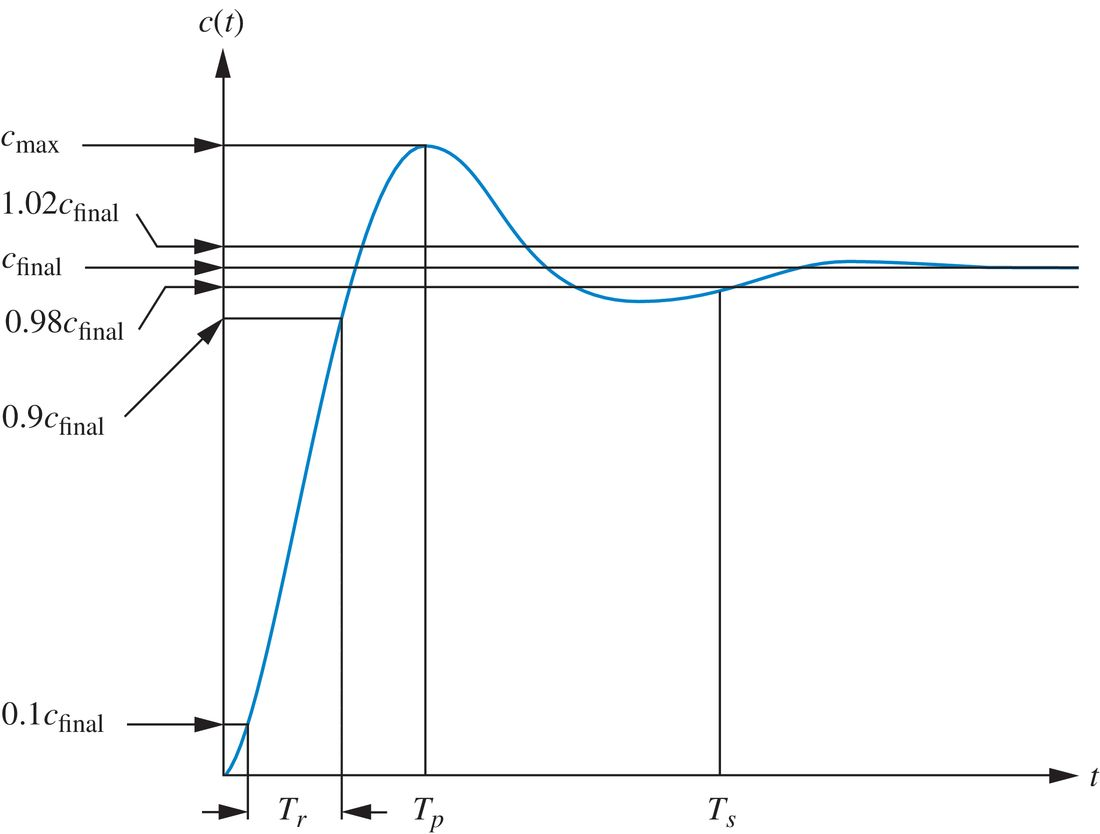
\includegraphics[width=0.7\textwidth]{fig_04_14.jpg}
  \caption{Transient performance specifications for an underdamped second-order
    step response.  (Adapted from Nise, Fig.~4.14.)}
  \label{fig:specs}
\end{figure}

% ---------------------------------------------------------------------------
\subsection{Peak Time}
\label{sec:tp}
% ---------------------------------------------------------------------------

\emph{Peak time}~$T_p$ is the time at which the step response first reaches
its maximum.  It is found by differentiating Eq.~\eqref{eq:step} and setting
the result to zero.  The derivative has the form of a sinusoid; its first zero
crossing after $t=0$ occurs at

\begin{equation}
  \boxed{T_p = \frac{\pi}{\omega_d}}
  \label{eq:Tp}
\end{equation}

Peak time is inversely proportional to the \emph{imaginary part} of the pole.

% ---------------------------------------------------------------------------
\subsection{Percent Overshoot}
\label{sec:pos}
% ---------------------------------------------------------------------------

\emph{Percent overshoot} (\%OS) is the amount by which the peak exceeds the
final value, expressed as a percentage of the final value.  Evaluating
Eq.~\eqref{eq:step} at $t = T_p$ and simplifying yields

\begin{equation}
  \boxed{\%OS = e^{-\pi\zeta/\sqrt{1-\zeta^2}} \times 100}
  \label{eq:pos}
\end{equation}

Because \%OS depends only on~$\zeta$, it is a pure measure of the damping
ratio (Figure~\ref{fig:os}).  Inverting Eq.~\eqref{eq:pos} gives the damping
ratio required to achieve a target overshoot:

\begin{equation}
  \zeta = \frac{-\ln(\%OS/100)}{\sqrt{\pi^2 + \ln^2(\%OS/100)}}
  \label{eq:zeta_from_pos}
\end{equation}

\begin{figure}[h]
  \centering
  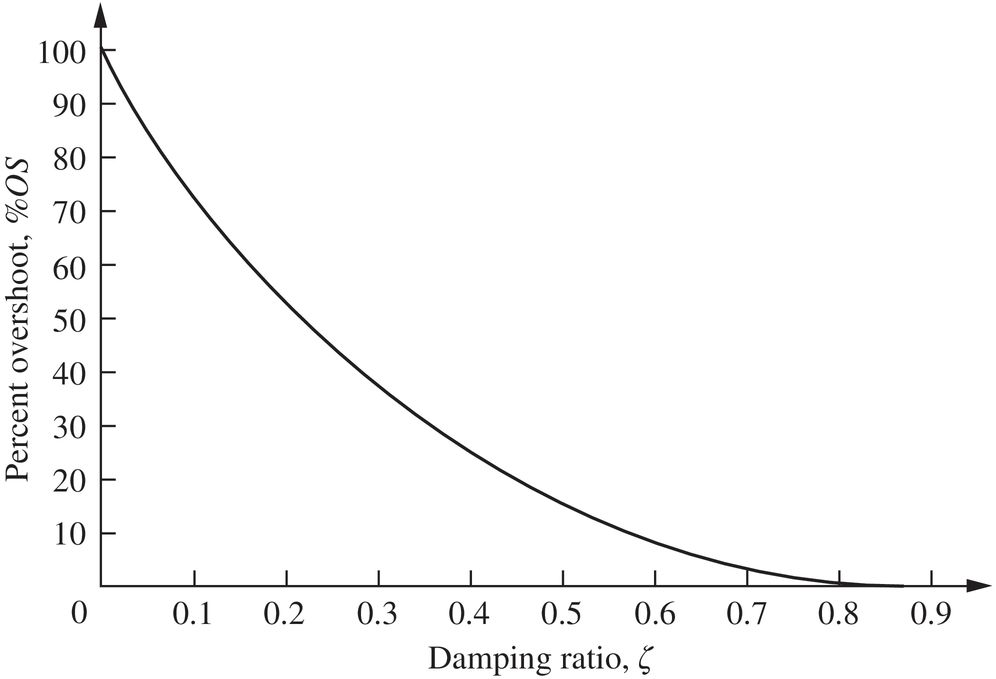
\includegraphics[width=0.55\textwidth]{fig_04_15.jpg}
  \caption{Percent overshoot as a function of damping ratio~$\zeta$.
    (Adapted from Nise, Fig.~4.15.)}
  \label{fig:os}
\end{figure}

% ---------------------------------------------------------------------------
\subsection{Settling Time}
\label{sec:ts}
% ---------------------------------------------------------------------------

\emph{Settling time}~$T_s$ is the time after which the response stays within
$\pm 2\%$ of its final value.  The exponential envelope of the step response
decays as $e^{-\sigma_d t}/\sqrt{1-\zeta^2}$.  Setting this envelope equal to
$0.02$ and solving gives the exact settling time; approximating the numerator
as a constant near $4$ across $0 \le \zeta \le 0.9$ yields the practical formula:

\begin{equation}
  \boxed{T_s \approx \frac{4}{\sigma_d} = \frac{4}{\zeta\omega_n}}
  \label{eq:Ts}
\end{equation}

Settling time is inversely proportional to the \emph{real part} of the pole.

% ---------------------------------------------------------------------------
\subsection{Rise Time}
\label{sec:tr}
% ---------------------------------------------------------------------------

\emph{Rise time}~$T_r$ is the time for the response to go from 10\% to 90\%
of its final value.  Unlike the other three metrics, no closed-form
expression relating $T_r$ to $\zeta$ and $\omega_n$ exists.

The normalized rise time $\omega_n T_r$ has been tabulated numerically; the
results are shown in Figure~\ref{fig:risetime}.  These values are well
approximated by the polynomial

\begin{equation}
  \omega_n T_r \approx 1.76\zeta^3 - 0.417\zeta^2 + 1.039\zeta + 1
  \qquad (0 < \zeta < 0.9, \text{ error} < 0.5\%)
  \label{eq:tr_poly}
\end{equation}

from which $T_r = (\omega_n T_r)/\omega_n$.

\begin{figure}[h]
  \centering
  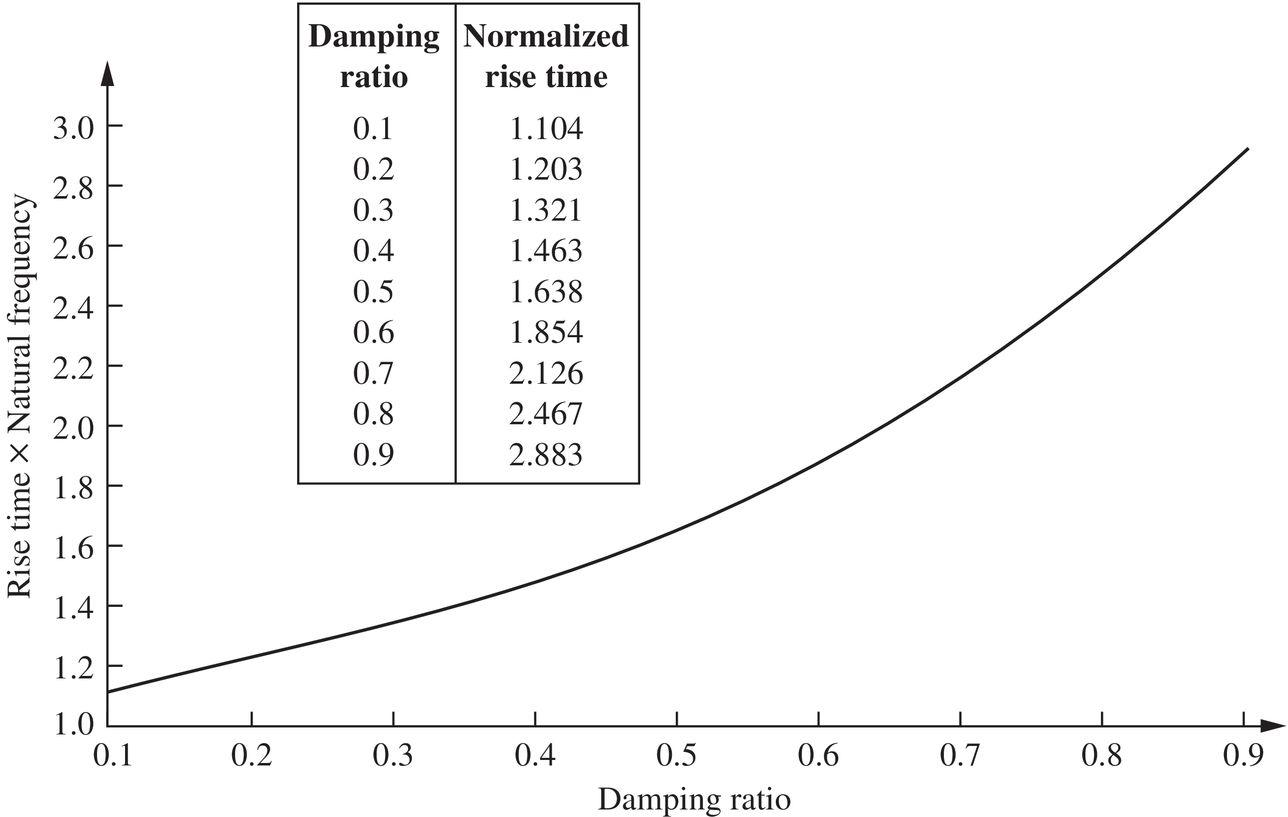
\includegraphics[width=0.70\textwidth]{fig_04_16.jpg}
  \caption{Normalized rise time~$\omega_n T_r$ versus damping ratio for an
    underdamped second-order step response.  The inset table gives exact
    numerical values.
    (Adapted from Nise, Fig.~4.16.)}
  \label{fig:risetime}
\end{figure}

% ---------------------------------------------------------------------------
\subsection{Pole Locations and Performance Specifications}
\label{sec:metrics_pole}
% ---------------------------------------------------------------------------

Equations~\eqref{eq:Tp}--\eqref{eq:Ts} reveal a direct and geometrically
elegant connection between pole location and transient performance.  For
underdamped poles at $s = -\sigma_d \pm j\omega_d$:

\begin{itemize}
  \item \textbf{Horizontal lines} (constant $\omega_d$) correspond to constant
    peak time $T_p = \pi/\omega_d$.
  \item \textbf{Vertical lines} (constant $\sigma_d$) correspond to constant
    settling time $T_s = 4/\sigma_d$.
  \item \textbf{Radial lines} from the origin (constant $\zeta = \cos\theta$,
    where $\theta$ is the angle from the negative real axis) correspond to
    constant percent overshoot.
\end{itemize}

Figure~\ref{fig:pole_geom} shows these relationships in the $s$-plane, and
Figure~\ref{fig:pole_motion} illustrates how moving the poles --- vertically,
horizontally, or radially --- changes the step response character in a
predictable way.

\begin{figure}[h]
  \centering
  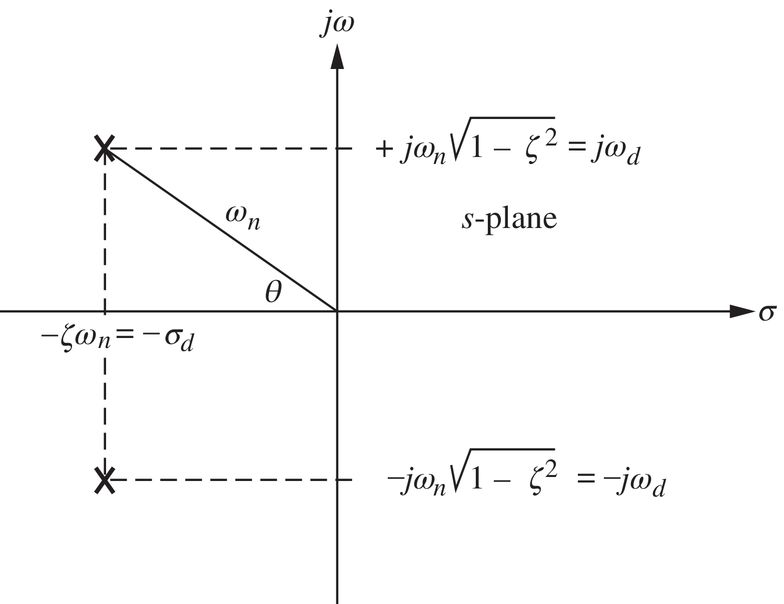
\includegraphics[width=0.52\textwidth]{fig_04_17.jpg}
  \caption{Geometry of an underdamped pole.  The radial distance is~$\omega_n$,
    the angle from the negative real axis gives $\zeta = \cos\theta$, and the
    Cartesian coordinates are $\sigma_d = \zeta\omega_n$ (real part) and
    $\omega_d$ (imaginary part).
    (Adapted from Nise, Fig.~4.17.)}
  \label{fig:pole_geom}
\end{figure}

\begin{figure}[h]
  \centering
  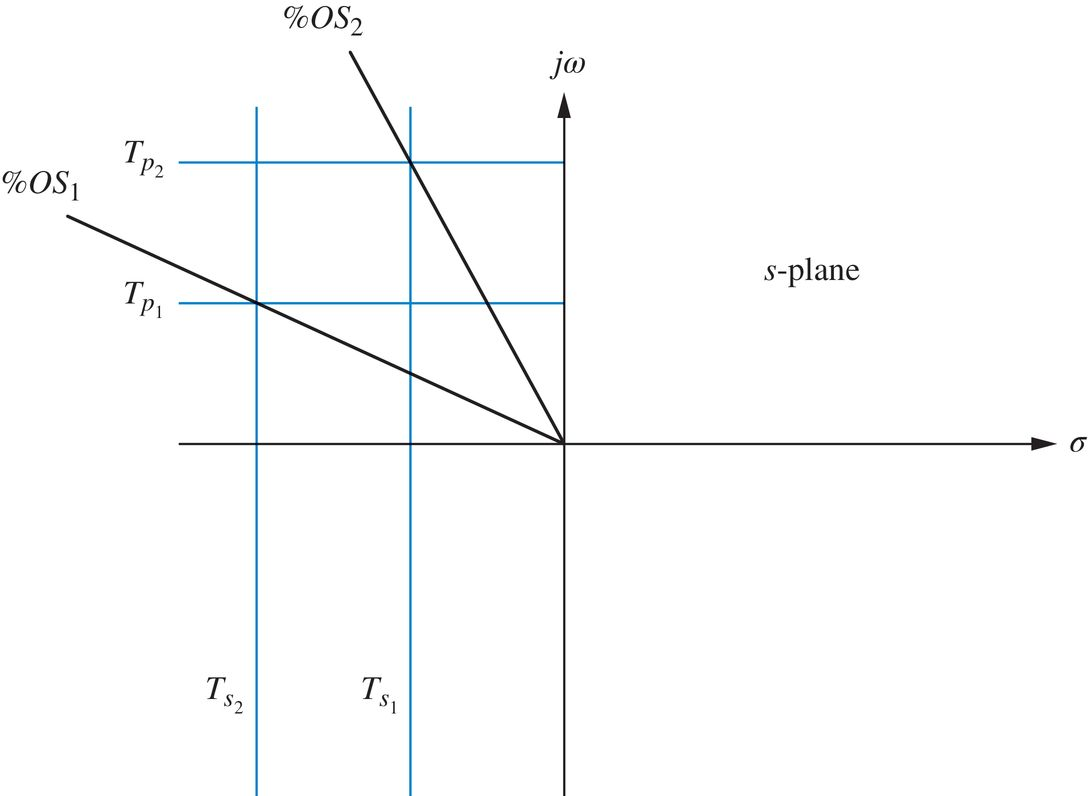
\includegraphics[width=0.80\textwidth]{fig_04_18.jpg}
  \caption{Lines of constant $T_p$, $T_s$, and \%OS in the $s$-plane.
    Moving a pole to the left shortens settling time; moving it upward
    shortens peak time (but increases frequency and overshoot for constant
    $\sigma_d$); moving along a constant-$\zeta$ line rescales both without
    changing overshoot.
    (Adapted from Nise, Fig.~4.18.)}
  \label{fig:lines}
\end{figure}

\begin{figure}[h]
  \centering
  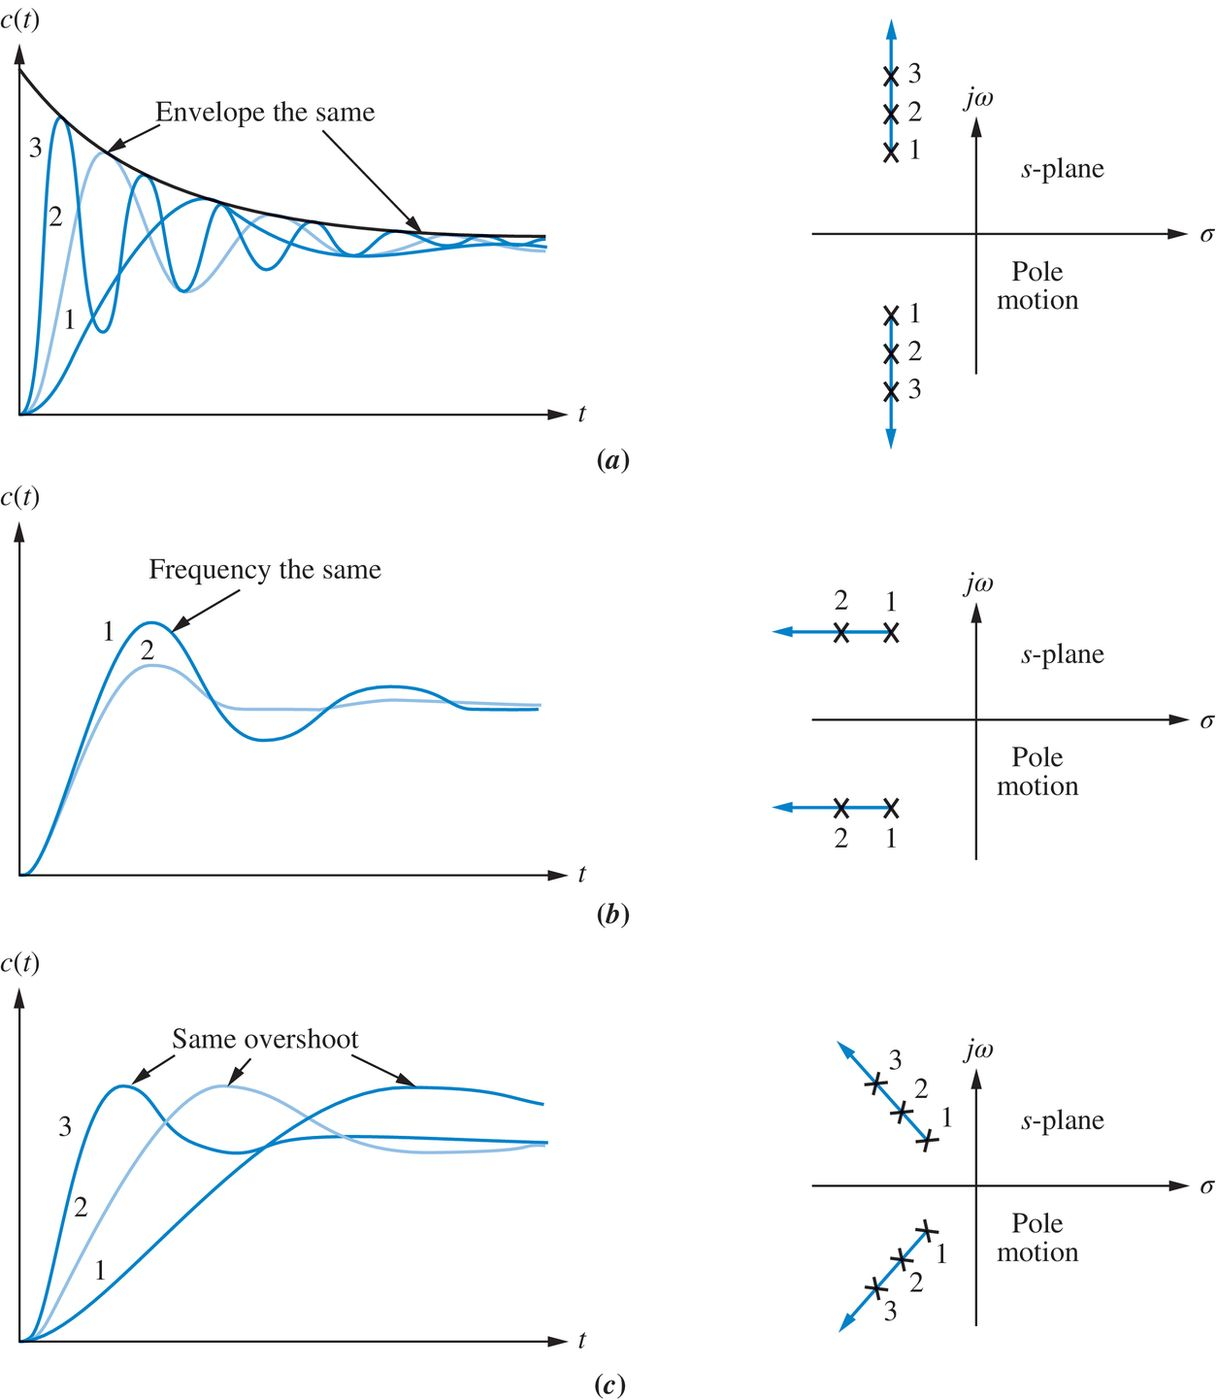
\includegraphics[width=0.80\textwidth]{fig_04_19.jpg}
  \caption{Step responses as poles are moved vertically (constant $\sigma_d$),
    horizontally (constant $\omega_d$), and along a constant-$\zeta$ radial line.
    (Adapted from Nise, Fig.~4.19.)}
  \label{fig:pole_motion}
\end{figure}

This geometric picture turns design into a mapping problem: given specifications
for $T_p$, $T_s$, and \%OS, draw the corresponding lines in the $s$-plane and
find the region where all constraints are satisfied.  The desired poles must
lie in that region.

% ===========================================================================
\section{Identifying Transfer Functions from Response Data}
\label{sec:testing}
% ===========================================================================

The performance metrics in Section~\ref{sec:metrics} are defined by the
\emph{shape} of the step response, not by how that response was produced.
This means they can be obtained in three equivalent ways:

\begin{description}
  \item[Analytically] from a known transfer function, using the formulas above.
  \item[Numerically] from any model --- including higher-order or nonlinear
    models --- using simulation.  In MATLAB, \texttt{stepinfo()} extracts all
    standard metrics from a computed step response, and \texttt{damp()} reports
    $\zeta$ and $\omega_n$ for each pole pair.
  \item[Experimentally] from measured data on the real system.  If the system
    behaves like a second-order underdamped model, measuring $T_p$, $T_s$, and
    \%OS from the step response gives $\zeta$, $\omega_n$, and $K_{dc}$, from
    which the transfer function can be reconstructed.
\end{description}

For a first-order system the identification is even simpler: the step response
steady-state value is $K_{dc}$, and the time at which the response reaches
$63\%$ of its final value is the time constant~$\tau = 1/a$.

This unification matters: the same specifications that describe an LTI model
analytically can also be measured on a physical system or evaluated from a
nonlinear simulation.  The metrics are the shared language across all three
approaches.

% ===========================================================================
\section{Higher-Order Systems: Let the Computer Work}
\label{sec:higher}
% ===========================================================================

All of the analysis above assumed a second-order system with no additional
poles and no zeros.  Real control systems are often higher order.

For higher-order models, we do not attempt the algebra by hand.  MATLAB
computes the step response and extracts performance metrics numerically:

\begin{verbatim}
  G = tf(num, den);          % define transfer function
  step(G)                    % plot step response
  info = stepinfo(G)         % Tp, Ts, Tr, %OS, etc.
  [wn, zeta, p] = damp(G)   % natural frequencies, damping ratios, poles
\end{verbatim}

The companion MATLAB script demonstrates these commands on first- and
second-order examples, and shows how to visualize the connection between
pole location and response.

% ===========================================================================
\section{Limitations: When the Formulas Do Not Apply}
\label{sec:limits}
% ===========================================================================

The performance metric formulas in Section~\ref{sec:metrics} apply
\emph{only} to the canonical second-order form:

\[
  G(s) = K_{dc}\,\frac{\omega_n^2}{s^2 + 2\zeta\omega_n s + \omega_n^2}
\]

They are \emph{not} valid when the system has:
\begin{itemize}
  \item \textbf{Additional poles.}  Extra poles add exponential components
    that distort the response.  If an additional pole is far enough to the
    left (typically $5\times$ farther than~$\sigma_d$), its contribution decays
    quickly and the second-order formulas remain approximately valid.  Otherwise,
    use MATLAB.
  \item \textbf{Zeros.}  A zero in the numerator changes the residues of the
    partial-fraction expansion, altering the amplitudes of each response
    component.  This can significantly modify overshoot and rise time relative
    to the zero-free case.
\end{itemize}

When in doubt, simulate: the metrics computed from the step response always
reflect the actual system behavior, regardless of order or zeros.

\end{document}
